

\tikzset{every picture/.style={line width=0.75pt}} %set default line width to 0.75pt        

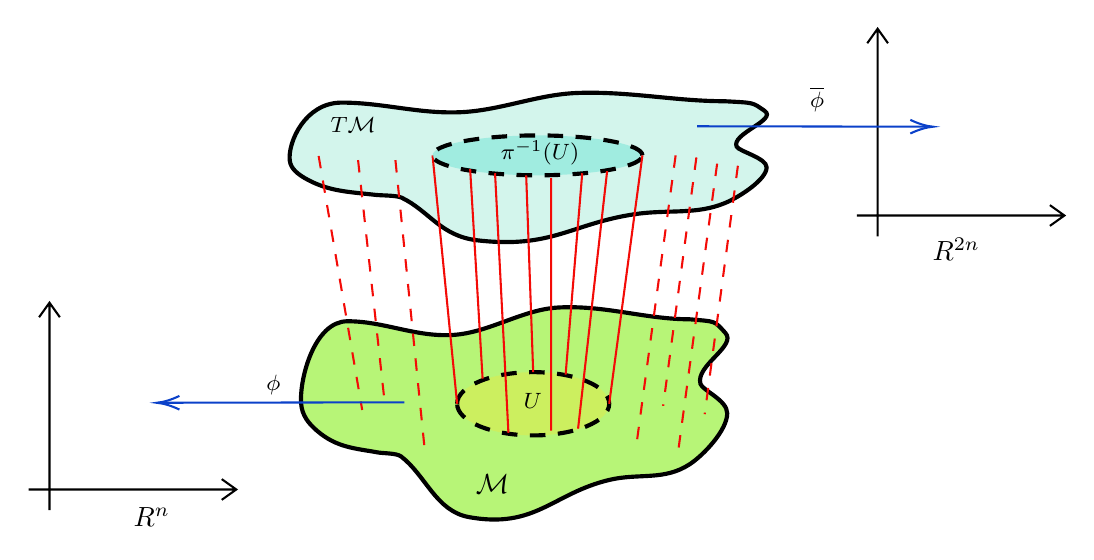
\begin{tikzpicture}[x=0.75pt,y=0.75pt,yscale=-1,xscale=1]
%uncomment if require: \path (0,351); %set diagram left start at 0, and has height of 351

%Shape: Boxed Bezier Curve [id:dp7555542346097139] 
\draw [fill={rgb, 255:red, 211; green, 245; blue, 236 }  ,fill opacity=1 ][line width=1.5]    (391.34,61.94) .. controls (367.37,61.94) and (345.22,57.03) .. (320.2,57.96) .. controls (300.91,58.67) and (282.94,66.54) .. (263.47,67.25) .. controls (243.27,67.98) and (226.53,62.6) .. (206.75,62.6) .. controls (189.05,62.6) and (180.8,81.91) .. (181.76,90.47) .. controls (182.21,94.49) and (185.77,97.27) .. (190.41,99.76) .. controls (201.06,105.48) and (210.83,105.65) .. (223.1,107.06) .. controls (225.93,107.38) and (233.27,107.27) .. (235.59,108.38) .. controls (248.94,114.76) and (254.4,126.91) .. (272.13,128.95) .. controls (308.22,133.11) and (317.45,120.88) .. (348.08,116.35) .. controls (363.96,114) and (377.58,116.74) .. (391.34,111.04) .. controls (398.74,107.97) and (411.53,99.55) .. (411.53,93.79) .. controls (411.53,89.32) and (398.16,86.03) .. (397.11,83.84) .. controls (394.13,77.68) and (416.9,70.96) .. (410.56,66.58) .. controls (404.35,62.3) and (405.76,62.75) .. (391.34,61.94) -- cycle ;
%Shape: Boxed Bezier Curve [id:dp6883735068899058] 
\draw [fill={rgb, 255:red, 158; green, 241; blue, 71 }  ,fill opacity=0.74 ][line width=1.5]    (374.5,167) .. controls (353.09,167) and (333.29,160.03) .. (310.94,161.34) .. controls (293.71,162.35) and (277.65,173.54) .. (260.26,174.55) .. controls (242.2,175.59) and (227.24,167.94) .. (209.57,167.94) .. controls (193.76,167.94) and (186.39,195.39) .. (187.24,207.57) .. controls (187.64,213.29) and (190.83,217.23) .. (194.97,220.77) .. controls (204.49,228.9) and (213.22,229.14) .. (224.18,231.15) .. controls (226.71,231.61) and (233.27,231.46) .. (235.34,233.04) .. controls (247.26,242.1) and (252.15,259.38) .. (267.99,262.28) .. controls (300.24,268.18) and (308.48,250.8) .. (335.85,244.36) .. controls (350.04,241.02) and (362.21,244.91) .. (374.5,236.81) .. controls (381.12,232.45) and (392.54,220.47) .. (392.54,212.28) .. controls (392.54,205.93) and (380.6,201.25) .. (379.66,198.13) .. controls (377,189.38) and (397.34,179.82) .. (391.68,173.6) .. controls (386.13,167.51) and (387.39,168.15) .. (374.5,167) -- cycle ;
%Shape: Ellipse [id:dp7913055919056734] 
\draw  [fill={rgb, 255:red, 245; green, 230; blue, 53 }  ,fill opacity=0.35 ][dash pattern={on 5.63pt off 4.5pt}][line width=1.5]  (262.41,207.7) .. controls (262.41,199.28) and (278.81,192.46) .. (299.05,192.46) .. controls (319.28,192.46) and (335.68,199.28) .. (335.68,207.7) .. controls (335.68,216.12) and (319.28,222.95) .. (299.05,222.95) .. controls (278.81,222.95) and (262.41,216.12) .. (262.41,207.7) -- cycle ;
%Straight Lines [id:da38840826454836663] 
\draw [color={rgb, 255:red, 243; green, 11; blue, 7 }  ,draw opacity=1 ][line width=0.75]    (250.56,88.02) -- (262.41,207.7) ;
%Shape: Ellipse [id:dp3372595327826894] 
\draw  [fill={rgb, 255:red, 119; green, 230; blue, 215 }  ,fill opacity=0.55 ][dash pattern={on 5.63pt off 4.5pt}][line width=1.5]  (351.68,88.02) .. controls (351.68,82.72) and (329.05,78.41) .. (301.12,78.41) .. controls (273.2,78.41) and (250.56,82.72) .. (250.56,88.02) .. controls (250.56,93.33) and (273.2,97.63) .. (301.12,97.63) .. controls (329.05,97.63) and (351.68,93.33) .. (351.68,88.02) -- cycle ;
%Straight Lines [id:da561591323588785] 
\draw [color={rgb, 255:red, 243; green, 11; blue, 7 }  ,draw opacity=1 ][line width=0.75]    (351.68,88.02) -- (335.68,207.7) ;
%Straight Lines [id:da690868976884767] 
\draw [color={rgb, 255:red, 243; green, 11; blue, 7 }  ,draw opacity=1 ][line width=0.75]    (334.68,95.63) -- (320.68,219.7) ;
%Straight Lines [id:da0643786859358153] 
\draw [color={rgb, 255:red, 243; green, 11; blue, 7 }  ,draw opacity=1 ][line width=0.75]    (280.68,96.63) -- (287.12,221.7) ;
%Straight Lines [id:da5276401921204039] 
\draw [color={rgb, 255:red, 243; green, 11; blue, 7 }  ,draw opacity=1 ][line width=0.75]    (307.72,98.81) -- (307.68,220.63) ;
%Straight Lines [id:da02591874235055658] 
\draw [color={rgb, 255:red, 243; green, 11; blue, 7 }  ,draw opacity=1 ][line width=0.75]    (268.68,94.63) -- (274.68,195.63) ;
%Straight Lines [id:da13234226839924923] 
\draw [color={rgb, 255:red, 243; green, 11; blue, 7 }  ,draw opacity=1 ][line width=0.75]    (295.68,97.63) -- (299.05,192.46) ;
%Straight Lines [id:da10881113373921192] 
\draw [color={rgb, 255:red, 243; green, 11; blue, 7 }  ,draw opacity=1 ][line width=0.75]    (322.68,96.63) -- (314.68,193.63) ;
%Straight Lines [id:da1622212363017358] 
\draw [color={rgb, 255:red, 243; green, 11; blue, 7 }  ,draw opacity=1 ][line width=0.75]  [dash pattern={on 4.5pt off 4.5pt}]  (367.68,88.02) -- (348.68,228.3) ;
%Straight Lines [id:da48330270456949853] 
\draw [color={rgb, 255:red, 243; green, 11; blue, 7 }  ,draw opacity=1 ][line width=0.75]  [dash pattern={on 4.5pt off 4.5pt}]  (377.68,89.02) -- (361.68,208.7) ;
%Straight Lines [id:da2990883543810654] 
\draw [color={rgb, 255:red, 243; green, 11; blue, 7 }  ,draw opacity=1 ][line width=0.75]  [dash pattern={on 4.5pt off 4.5pt}]  (195.68,88.3) -- (216.68,210.7) ;
%Straight Lines [id:da95060641908313] 
\draw [color={rgb, 255:red, 243; green, 11; blue, 7 }  ,draw opacity=1 ][line width=0.75]  [dash pattern={on 4.5pt off 4.5pt}]  (214.68,90.3) -- (227.68,208.7) ;
%Straight Lines [id:da7748858791112593] 
\draw [color={rgb, 255:red, 243; green, 11; blue, 7 }  ,draw opacity=1 ][line width=0.75]  [dash pattern={on 4.5pt off 4.5pt}]  (232.68,90.3) -- (246.68,228.7) ;
%Straight Lines [id:da23543355149656475] 
\draw [color={rgb, 255:red, 243; green, 11; blue, 7 }  ,draw opacity=1 ][line width=0.75]  [dash pattern={on 4.5pt off 4.5pt}]  (387.68,92.02) -- (368.68,232.3) ;
%Straight Lines [id:da252934263423064] 
\draw [color={rgb, 255:red, 243; green, 11; blue, 7 }  ,draw opacity=1 ][line width=0.75]  [dash pattern={on 4.5pt off 4.5pt}]  (397.68,93.02) -- (381.68,212.7) ;
%Shape: Axis 2D [id:dp028583688594270185] 
\draw  (56,249) -- (156,249)(66,159) -- (66,259) (149,244) -- (156,249) -- (149,254) (61,166) -- (66,159) -- (71,166)  ;
%Shape: Axis 2D [id:dp8970413200540654] 
\draw  (455,117) -- (555,117)(465,27) -- (465,127) (548,112) -- (555,117) -- (548,122) (460,34) -- (465,27) -- (470,34)  ;
%Straight Lines [id:da828009539651172] 
\draw [color={rgb, 255:red, 11; green, 65; blue, 201 }  ,draw opacity=1 ]   (237,207) -- (119.68,207.21) ;
\draw [shift={(117.68,207.22)}, rotate = 359.9] [color={rgb, 255:red, 11; green, 65; blue, 201 }  ,draw opacity=1 ][line width=0.75]    (10.93,-3.29) .. controls (6.95,-1.4) and (3.31,-0.3) .. (0,0) .. controls (3.31,0.3) and (6.95,1.4) .. (10.93,3.29)   ;
%Straight Lines [id:da45797751736499215] 
\draw [color={rgb, 255:red, 11; green, 65; blue, 201 }  ,draw opacity=1 ]   (378,74) -- (489.68,74.21) ;
\draw [shift={(491.68,74.22)}, rotate = 180.11] [color={rgb, 255:red, 11; green, 65; blue, 201 }  ,draw opacity=1 ][line width=0.75]    (10.93,-3.29) .. controls (6.95,-1.4) and (3.31,-0.3) .. (0,0) .. controls (3.31,0.3) and (6.95,1.4) .. (10.93,3.29)   ;

% Text Node
\draw (270,240.4) node [anchor=north west][inner sep=0.75pt]    {$\mathcal{M}$};
% Text Node
\draw (282,79.4) node [anchor=north west][inner sep=0.75pt]  [font=\footnotesize]  {$\pi ^{-1}( U)$};
% Text Node
\draw (293,201.4) node [anchor=north west][inner sep=0.75pt]  [font=\footnotesize]  {$U$};
% Text Node
\draw (200,68.4) node [anchor=north west][inner sep=0.75pt]  [font=\footnotesize]  {$T\mathcal{M}$};
% Text Node
\draw (105,256.4) node [anchor=north west][inner sep=0.75pt]    {$\mathbb{R}^{n}$};
% Text Node
\draw (490,126.4) node [anchor=north west][inner sep=0.75pt]    {$\mathbb{R}^{2n}$};
% Text Node
\draw (169,192.4) node [anchor=north west][inner sep=0.75pt]  [font=\footnotesize]  {$\phi $};
% Text Node
\draw (431,53.4) node [anchor=north west][inner sep=0.75pt]  [font=\footnotesize]  {$\overline{\phi }$};


\end{tikzpicture}
